\section{Grupos funcionales y jerarquías}

En esta fase, una vez definidos los elementos de datos y funcionales, vamos a
organizarlos agrupándolos en unidades funcionales que nuestras personas el
trabajo en una tarea y la transición entre tareas. Para mostrarlo de manera más
visual hemos realizado un diagrama en árbol, para el que hemos usado el
programa \underline{\href{https://www.drawio.com/}{draw.io}}. Tras un análisis, 
hemos obtenido el resultado que observamos en la figura \ref{fig:jerarquias}, el cuál explicamos a 
continuación:
\begin{figure}[H]
      \centering
      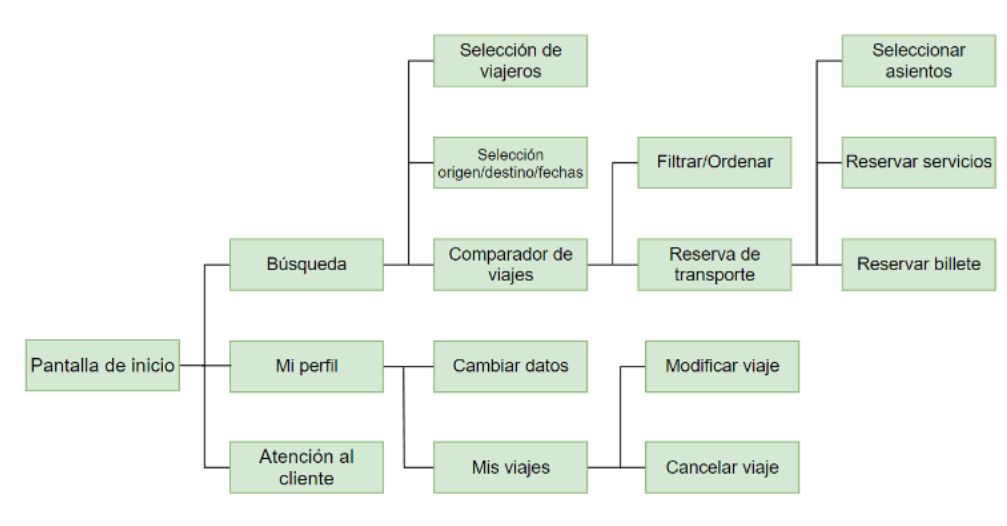
\includegraphics[width=0.8\linewidth]{./Imagenes/jerarquia.png}
      \caption{Diagrama de jerarquías de funciones}
      \label{fig:jerarquias}
\end{figure}

\begin{itemize}
    \item La pantalla de inicio contiene los elementos de búsqueda, atención al cliente y mi perfil.
    \item El elemento de búsqueda es el componente principal por lo que ocupa gran espacio en la interfaz. Al usarla podrás realizar la selección de origen destino y/o fechas, así como de los viajeros. Estas opciones sirven como filtro a la hora de realizar la comparación, que se muestra a continuación.
    \item En el apartado de Comparador de viajes puedes ver todos los que cumplen los criterios anteriormente mencionados. Además puedes cambiar los filtros anteriores y/u ordenarlos según distintos criterios. Además podrás seleccionar si quieres que se muestren solo los viajes accesibles para personas con discapacidad física.
    \item Una vez te interesas por un viaje, pasarás al apartado de Reserva de transporte. Aquí se mostrarán todos los datos de manera clara, como se marcó en los requisitos, además de poder elegir los asientos y realizar la propia reserva del billete.
    \item En el apartado Mi perfil se puede cambiar los datos del usuario (nombre, correo, teléfono, etc) además de poder ver las reservas pasadas, pudiendo tanto cancelar el viaje como modificarlo (fecha u hora, siempre que lo permita la compañía).
    \item Como se comentó en el apartado anterior, se podrá acceder al apartado de atención al cliente desde cualquier punto de la aplicación.
    \item Un principio que podría ser útil para la aplicación es la programación orientada a objetos, debido a que tenemos distintas partes que podrían ser encapsuladas en éstos, como son los viajes.
    \item En cuanto a los patrones, uno de lo que podría usarse sería el patrón Singleton ya que asegura que cada clase tenga una única instancia, controla el acceso a cada recurso y tiene un control estricto de las variables disponibles.
\end{itemize}

\subsection{Orden general en que se usarán los elementos}

\begin{enumerate}

      \item Cambiar la configuración de idioma y moneda.
      \item Acceder a \textit{Atención al cliente} desde la \textit{Página principal}.
      \item Acceder a \textit{Perfil} desde la \textit{Página principal}.
      \item Funcionalidad principal: comparar distintas opciones de transportes según las
            necesidades.

\end{enumerate}

\subsection{Principios y patrones usados}

\begin{itemize}

      \item \textbf{Principio de proximidad.} Este principio nos dice que cuando ciertos elementos están próximos, el cerebro interpreta
            que están relacionados. Esto facilita tanto el aprendizaje como la memoribiliadad de cara al usuario. Este principio lo usamos en prácticamente
            todas las ventanas, ya que la mayoría poseen varios botones u opciones relacionadas que son agrupables.
      \item \textbf{Consistencia interna.} Dentro de la aplicación mantenemos todos los elementos que posean la misma funcionalidad con apariencias iguales
            o similares. Esto lo hemos aplicado en el los fondos de la aplicación, en el uso de las \textit{Cards} para los viajes, en la fuente de letra, los
            botones, etc. De esta manera, se facilita que el usuario perciba las potencialidades de los elementos de la interfaz.
      \item \textbf{Consistencia externa.} 
      \item \textbf{Principio de visibilidad.}
      \item \textbf{Ley de Hick.} Esta ley nos dice que el tiempo que hay que invertir para tomar una decisión incrementa con el número de opciones disponibles y la complejidad
            de éstas. Por eso, es importante dividir las tareas complejas en varios pasos. Esto lo aplicamos al realizar la reserva de un viaje, ya que ésta cuenta de varios
            pasos (\textit{Comparador}, donde se muestran todos los viajes disponibles; \textit{Reserva}, donde el usuario pone los datos adicionales del viaje, como los asientos
            o el resto de servicios; \textit{Pago}, donde el usuario rellena los datos referentes al pago para confirmar la reserva).
      \item \textbf{Efecto Zeigarnik.}
      \item \textbf{Principio de libertad y control del usuario.} En todos los aspectos intentamos dar el máximo control y libertad al usuario. Esto lo hacemos poniendo un botón para volver a la anterior
            pantalla en la mayoría de páginas y, por ejemplo, permitiendo la modificación o cancelación de las reservas hechas.
      \item \textbf{Principio de cierre.} Este principio nos dice que nuestro cerebro tiene tendencia a identificar patrones secuenciales, que constan de planteamiento, desarrollo y cierre,
            el cuál debe ser natural, una continuación del proceso que estábamos siguiendo. Este principio lo usamos por ejemplo en las pantallas en las que hay que hacer \textit{scroll} hacia abajo,
            dejando algún elemento entrecortado para mostrar al usuario que hay más elementos debajo.
      \item \textbf{Ley de Fitts.} 
      \item \textbf{Regla del \textit{peak-end}} Esta regla es un sesgo cognitivo que nos dice que los momentos intensos y los momentos finales de
            de una experiencia tienen gran importancia al recordar eventos pasados, por eso es importante cuidar estos momentos. Al finalizar un proceso laborioso como
            puede ser el de reserva de un viaje, mostramos una pantalla de que ha sido correctamente reservado, dando una sensación de tranquilidad al usuario
            al final del proceso.

\end{itemize}
